\documentclass[output=paper]{langsci/langscibook}
\ChapterDOI{10.5281/zenodo.3972868}
\author{James Baker\affiliation{University of Cambridge}}
\title{Rethinking split intransitivity}

% \chapterDOI{} %will be filled in at production

\abstract{This chapter presents a development of \citegen{Perlmutter1978}
    \isi{unaccusative hypothesis}. It argues that the verbal domain should be
    considered to comprise an ordered series of functional heads\is{functional items} here termed
    the VISCO hierarchy, and that this approach permits an improvement
    understanding of split intransitive behaviours. The history of research
    into unaccusativity and split intransitivity is considered, with the
    strengths and weaknesses of the proposals made by
    \textcite{Perlmutter1978}, \textcite{Burzio1986},
    \textcite{LevinRappaportHovav1995} and others discussed and compared to the
    VISCO approach. The VISCO hierarchy is also compared to the hierarchy
    proposed in \textcite{Ramchand2008} and discussed in relation to the work
    of \textcite{Sorace2000}. Issues such as difficulties in classifying
    unergatives/unaccusatives within a single language, apparent variation
    between languages, and the problem of syntax–semantics linking are all
considered.}

\maketitle

\begin{document}\glsresetall

\section{Introduction}

The purpose of this chapter is to present, in overview, a new approach to the
phenomena of \enquote{split intransitivity} – phenomena where different sorts
of intransitive predicates allow or disallow different syntactic behaviours.
Specifically, I discuss this new approach in the context of a comparison to
some of the major previous contributions in this area. Some strengths and
weaknesses of these various existing approaches are critically evaluated, with
arguments for how the new approach overcomes some of the weaknesses of those
previous whilst retaining their important insights.

Examples of split intransitive phenomena include those presented in (\ref{ex:baker:1}--\ref{ex:baker:4}),
from \ili{English}, and (\ref{ex:baker:5}--\ref{ex:baker:7}), from other languages. In each case, different verbs
exhibit different behaviours in relation to the constructions in question:

\ea\label{ex:baker:1} The causative alternation
    \ea
        \ea[]{The lollipops melted.}
        \ex[]{Lucy melted the lollipops.}
        \z
    \ex
        \ea[]{The window broke.}
        \ex[]{Chris broke the window.}
        \z
    \ex
        \ea[]{Harry coughed.}
        \ex[*]{Sarah coughed Harry. [intended meaning: \enquote*{Sarah made Harry cough.}]}
        \z
    \ex
        \ea[]{The pickpocket talked.}
        \ex[*]{The police talked the pickpocket. [intended meaning: \enquote*{The police made the pickpocket talk.}]}
        \z
    \z
\ex Prenominal past \isi{participles}
    \ea[]{the melted lollipops}
    \ex[]{the broken window}
    \ex[]{the recently arrived recruits}
    \ex[*]{the coughed man}
    \ex[*]{the talked pickpocket}
    \ex[*]{the played cricketers}
    \z
\ex \emph{out}-prefixation
    \ea[]{Lucy outtalked/outworked/outplayed/outswam/outran Chris.}
    \ex[*]{Lucy outremained/outdied/outcame/outarrived Chris.}
    \z
\ex\label{ex:baker:4} V \emph{one's way into}
    \ea[]{%
        Lucy talked her way into the building.}
    \ex[]{%
        Chris worked his way into the upper echelons of university administration.
    }
    \ex[]{%
        Wayne played his way into the quarter-final.
    }
    \ex[*]{Jessica died her way into the cemetery.}
    \ex[*]{The train arrived its way into the station.}
    \z
\ex Auxiliary selection (German)\label{ex:baker:5}
    \ea
        \gll Hans \textit{ist} gegangen.\\
            Hans is   gone\\
        \glt \enquote*{Hans went.}\\
    \ex
        \gll Hans \textit{hat} gespielt.\\
        Hans has   played\\
        \glt \enquote*{Hans played.}\\
    \z
\ex \emph{Ne}-cliticisation (Italian)
    \ea[]{%
        \gll Ne   arrivano   molti.\\
            of-them arrive-\Tpl{} many-\M.\Pl{}\\
        \glt \enquote*{(Of them,) many arrived.} \parencite[221]{Bentley2004}}
    \ex[*]{%
        \gll Ne   studiano   molti.\\
            of-them study-\Tpl{} many-\M.\Pl{}\\
        \glt \enquote*{(Of them,) many studied.} \parencite[222]{Bentley2004}}
    \z
\ex\label{ex:baker:7} Case marking (\ili{Georgian})
    \ea
        \gll    Rezo   gamoizarda.\\
                Rezo.\Nom{}   he.grew.up\\
        \glt    \enquote*{Rezo grew up.} \parencite[293]{Harris1982}
    \ex
        \gll    Nino-\textit{m} daamtknara.\\
                Nino-\Erg{} she.yawned\\
        \glt    \enquote*{Nino yawned.} \parencite[147]{Harris1981}
    \z
\z
The new approach to syntactic structure proposed to account for these
phenomena, here labelled the VISCO hierarchy, is presented
in~\sectref{sec:visco}.  In \sectref{sec:unacc}, I then compare the VISCO approach with previous
approaches  following \citeapos{Perlmutter1978} \isi{unaccusative hypothesis}. I
argue that the VISCO approach overcomes a number of the problems of its
predecessors, though I shall also stress that it should be seen as a
development of ideas already in the literature, not something in radical
opposition to them. \sectref{sec:baker:conclusion} concludes.

\section{The VISCO hierarchy}\label{sec:visco}

In \textcite{Baker2016,Baker2018,Baker2019} I posit variants on the following
structure for the thematic domain (equivalent to \emph{v}P), termed the
\enquote{thematic functional hierarchy} (\glsunset{TFH}\gls{TFH}) or the
\enquote{VISCO hierarchy} after the initials of the five heads it
comprises, see~\Cref{fig:baker:2}.\footnote{The reader may note similarities between the VISCO approach
    and that of \citet{Ramchand2008}. I compare the two approaches briefly here
    in \sectref{sec:baker:3.4.2}, and in more detail in \citet{Baker2018}. Note that the variant
of this hierarchy in \textcite{Baker2018}, comprising a slightly different
set of heads is called the \enquote{VICTR hierarchy}.}

\begin{figure}
    \caption{The thematic functional hierarchy\label{fig:baker:2}}
    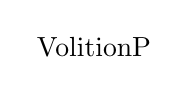
\begin{tikzpicture}[baseline=(root.base)]
        \Tree 	[.\node(root){VolitionP};
                    Volition
                    [.InitiationP
                        Initiation
                        [.StateP
                            State
                            [.ChangeP
                                Change
                                [.OrientedP
                                    Oriented
                                    VP
                                ]
                            ]
                        ]
                    ]
                ]

    \end{tikzpicture}
\end{figure}

Arguments may be merged in the specifier positions of any of these heads and
they gain their thematic interpretation from the positions in which they are
merged. I describe an argument merged in Spec,VolitionP as bearing
\textsc{θ-volition}, one merged  in Spec,InitiationP as bearing
\textsc{θ-initiation}, and so forth. A single argument may be merged in
multiple positions and hence bear multiple \enquote{roles}.\footnote{This is of
    course at odds with the traditional analysis of \isi{thematic roles} and argument
    \isi{movement} going back to the government and binding (\glsunset{GB}\gls{GB}) framework. In \gls{GB},
    arguments must have exactly one thematic role, which is assigned to them on
    the basis of its D-structure position (in minimalist terms, its first-merge
    position); \isi{movement} to positions in which \isi{thematic roles} may be assigned is
barred. However, there seems to be no a priori reason why these
principles should necessarily hold, and a minimalist grammar may reasonably
reject them.} For example, in the sentence in~\Cref{fig:baker:2lucy}
\emph{Lucy} (a volitional initiator undergoing a change of location) bears
\textsc{θ-volition\,+\,θ-initiation\,+\,θ-change}.\footnote{In this and all
    subsequent trees I omit all structure outside of the thematic domain, and
represent V only in its first-merge position.}

\begin{figure}
\caption{An example of thematic role assignment\label{fig:baker:2lucy}}
\raggedright Lucy is coming.\\
    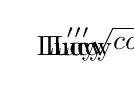
\begin{tikzpicture}[baseline]
        \Tree 	[.VolitionP
                    [.DP \edge[roof]; \node (fin) {Lucy}; ]
                    [.Volition$'$
                        Volition
                        [.InitiationP
                            [.DP \edge[roof]; \node (int) {Lucy}; ]
                            [.Initiation$'$
                                Initiation
                                [.StateP
                                    State
                                    [.ChangeP
                                        [.DP \edge[roof]; \node (sbj) {Lucy}; ]
                                        [.Change$'$
                                            Change
                                            [.OrientedP
                                                Oriented
                                                [.VP \edge[roof]; $\sqrt{come}$ ]
                                            ]
                                        ]
                                    ]
                                ]
                            ]
                        ]
                    ]
                ]

    \end{tikzpicture}
\end{figure}

The five VISCO heads are determined on the basis of the main features which I\largerpage
have deemed to be determinants of split intransitive behaviour in the languages
I have studied in this regard: [$\pm$\Volition{}], [$\pm$\Initiation{}],
[$\pm$\State{}], [$\pm$\Change{}] and [$\pm$\Oriented{}]. (These languages include
English, the Western European languages discussed by \citet{Sorace2000}, and
various languages with \enquote{split-S} case and/or agreement systems,
including particularly \ili{Basque} and \ili{Georgian}; see\linebreak
\citealt{Baker2016,Baker2018,Baker2019} for further discussion.) Encoding each
of these features on separate heads is in line with the principle \enquote{one
feature–one head} of the cartographic programme (see
\citealt{vanCraenenbroeck2009} and discussion in \citealt{Baker2018}) and is
also supported by evidence for the hierarchical ordering of the features
(partially discussed here in \sectref{sec:baker:3.4.6}; see \citealt{Baker2018} for more in-depth
discussion).

The \Volition{} head, which distinguishes whether an event is volitionally
controlled or not – as opposed to \Initiation{}, which expresses causation
independently of volition – allows us to capture behaviours such as the
following (from \ili{Tibetan}):

\ea \ili{Tibetan} \parencite[132]{DeLancey1984}
    \ea
        \gll Ŋa-\textit{s} Seattle-la phyin-pa-yin.\\
        \Fsg-\Erg{}  Seattle-to  went-\Prf.\Vol\\ \hfill [$+$\Volition{}]
        \glt \enquote*{I went to Seattle.}\\
    \ex
        \gll Ŋa-\textit{∅} śi-byuŋ.\\
        \Fsg-\Abs{}    die-\Prf.\Invol\\ \hfill[$–$\Volition{}]
        \glt \enquote*{I died.}
    \z
\z
\Volition{} seems to be marginally active in split intransitive behaviours in
English -- note the following contrasts, where the [$+$\Volition{}] sentences are
more strongly accepted with the diagnostics than the [$-$\Volition{}] ones:

\ea
    \ea[]{%
    Lucy outplayed/outtalked/outran Chris.\hfill[$+$\Volition{}]}
    \ex[?]{%
    Lucy outcoughed/outtrembled/outskidded Chris.\hfill[$-$\Volition{}] }
    \z
\z

\ea
    \ea {}[$+$\Volition{}]
        \ea[]{Lucy played a play.}
        \ex[]{Lucy talks the talk.}
        \ex[]{Lucy ran a run.}
        \z
    \ex {}[$-$\Volition{}]
        \ea[?]{Lucy trembled a tremble.}
        \ex[?]{Lucy skidded a skid.}
        \z
    \z
\z
The \Initiation{} and \Change{} heads capture for example the distinction made
between [$–$\Initiation{}, $+$\Change{}] intransitives which allow the causative
alternation in \ili{English}, and [$+$\Initiation{}] or [$–$\Change{}] verbs which do not
(an analysis modified from \citealt{Ramchand2008}):\largerpage[-1]

\ea The causative alternation:
    \ea
        \ea[]{The lollipops melted.\hfill[$-$\Initiation{}, $+$\Change{}]}
        \ex[]{Lucy melted the lollipops.}
        \z
    \ex
        \ea[]{Chris arrived.\hfill[+\Initiation{}, $+$\Change{}]}
        \ex[*]{Lucy arrived Chris. [intended meaning: \enquote*{Lucy made Chris
        arrive.}]}
        \z
    \ex
        \ea[]{The vase remained on the table.\hfill[$-$\Initiation{}, –\Change{}]}
        \ex[*]{Harry remained the vase. [intended meaning: \enquote*{Harry made the vase remain}]}
        \z
    \ex
        \ea[]{The pickpocket talked.\hfill[+\Initiation{}, $-$\Change{}]}
        \ex[*]{The police talked the pickpocket. [intended meaning: \enquote*{the police made the pickpocket talk}]}
        \z
    \z
\z
The \Change{} head, alongside \State{}, further allows us to identify three classes
of intransitives in \ili{English}. [$–$\State{}, $–$\Change{}] verbs allow constructions
such as the following, which do not generally occur with [$+$\Change{}] verbs:

\ea
    \ea {}[$-$\State{}, $-$\Change{}]
        \ea[]{Lucy talked her way into the room.}
        \ex[]{talker}
        \z
    \ex {}[$+$\Change{}]
        \ea[*]{Lucy arrived her way into the room.}
        \ex[*]{melter, *arriver}
        \z
    \z
\z
[$+$\Change{}] intransitives, on the other hand can generally occur as prenominal
past \isi{participles}, but [$-$\Change{}] intransitives do not:

\ea
    \ea {}[$+$\Change{}]
        \ea[]{the melted ice}
        \ex[]{the recently arrived recruits}
        \z
    \ex {}[$-$\Change{}]
        \ea[*]{the coughed man}
        \ex[*]{the talked professor}
        \z
    \z
\z
[$+$\State{}] intransitives form a distinct class, allowing neither set of
constructions:

\ea
    \ea[*]{Lucy stayed her way into the room.}
    \ex[*]{stayer}
    \ex[*]{the stayed man}
    \z
\z
This is evidence for the operation of the [$\pm$\State{}] feature.

Finally, I employ the head labelled \Oriented{} to account for the distinction
between (inherently) telic verbs like \emph{arrive} and \emph{tear}
([$+$\Oriented{}]) and atelic verbs like \emph{melt}, \emph{stay} and
\emph{talk} ([$-$\Oriented{}]). Only the latter readily occur with \emph{for
hours}:

\ea
    \ea {}[$+$\Oriented{}]
        \ea[*]{Lucy arrived for hours.}
        \ex[*]{The cloth tore for hours.}
        \z
    \ex {}[$-$\Oriented{}]
        \ea{The ice melted for hours.}
        \ex{Lucy stayed for hours.}
        \ex{Chris talked for hours.}
        \z
    \z
\z
In the following section I compare the VISCO hierarchy approach to split
intransitivity in relation to previous work on the topic.

\section{The VISCO hierarchy and the unaccusative\is{unaccusativity} hypothesis}\label{sec:unacc}

\subsection{Introduction}\label{sec:baker:3.1}

In this section I discuss the VISCO hierarchy in relation specifically to the
major existing approach to \isi{split intransitivity}, the \enquote{unaccusative
hypothesis}, in its various forms. The \isi{unaccusative hypothesis} was first
introduced in \citet{Perlmutter1978} and has been refined in much subsequent
work. \sectref{sec:baker:3.2} overviews the \isi{unaccusative hypothesis} as originally formulated. \sectref{sec:baker:3.3}
identifies one major strength of the \isi{unaccusative hypothesis} and considers how
this is retained in the VISCO approach. §§\ref{sec:baker:3.4} and \ref{sec:baker:3.5} then identify two
important weaknesses of Perlmutter’s original proposal, and discuss various
attempts to overcome these -- it is argued that these, in turn, have
weaknesses which can be overcome in the VISCO model.

\subsection{The origins of the unaccusative\is{unaccusativity} hypothesis}\label{sec:baker:3.2}

It was \citeapos{Perlmutter1978} hugely influential article that first brought
split intransitivity to the fore of discussion in generative linguistics.
Working within the framework of \isi{relational grammar}, Perlmutter formulated the
following hypothesis:

\ea\label{ex:unacc}The \isi{unaccusative hypothesis} \parencite[160]{Perlmutter1978}\\\enquote{Certain
    intransitive clauses have an initial 2 but no initial
    1.}
\z
\enquote{1} and \enquote{2} in \isi{relational grammar} terms refer to primitives of
grammatical relations. A \enquote{final 1} is a \enquote{surface subject}; a
\enquote{final 2} a \enquote{surface direct object}. In an ordinary active
transitive sentence, the final 1 is also an \enquote{initial} 1, and the final
2 an \enquote{initial} 2.  However, arguments may change relation between the
initial and final levels (\enquote{strata}); hence for example in the \isi{passive}
the initial 2 is \enquote{advanced} to become a final 1 (the surface subject).
The idea in (\ref{ex:unacc}), therefore, is that \emph{certain intransitive
    clauses have an argument which bears the same relation as the direct object
    of transitive clauses}. As in the \isi{passive}, however, this argument is
    advanced to the final 1\slash\enquote{surface subject} position, in accordance
    with the \enquote{final 1 law} which states that all clauses must have a
    final 1 \parencite[160]{Perlmutter1978}.

Perlmutter divided intransitive predicates into two groups, terming them
\enquote{unergatives} (clauses with an initial 1) and \enquote{unaccusatives}
(clauses with an initial 2). The basis of this division was semantic, though it
was encoded in the syntax (see \citealt{LevinRappaportHovav1995}: 4–5). On
Perlmutter’s scheme, the division of intransitives into unergatives and
unaccusatives was as follows (see \citealt{Perlmutter1978}: 162–5 for fuller
lists and discussion):

\ea\label{ex:19.19} Unergatives
    \ea Willed or volitional acts: e.g. \emph{work, play}, \emph{speak}, \emph{swim}, \emph{walk} \dots{} (includes manner-of-speaking verbs e.g. \emph{whisper}, \emph{shout} and predicates describing sounds made by animals e.g. \emph{bark}, \emph{neigh})
    \ex Certain involuntary bodily processes: e.g. \emph{cough}, \emph{sneeze} \dots{}
    \z
\z

\ea\label{ex:19.20} Unaccusatives
    \ea Predicates expressed by adjectives in English
    \ex Predicates whose argument is a semantic patient: e.g. \emph{burn}, \emph{fall}, \emph{slide}, \emph{drown}, \emph{sit} \dots{} (includes inchoatives e.g. \emph{melt}, \emph{freeze} \dots{})
    \ex Predicates of existing and happening: e.g. \emph{exist}, \emph{happen}, \emph{disappear} \dots{}
    \ex Non-voluntary emission of stimuli that impose on the senses: e.g. \emph{shine}, \emph{sparkle} \dots{}
    \ex Aspectual predicates: e.g. \emph{begin}, \emph{stop} \dots{}
    \ex Duratives: e.g. \emph{last}, \emph{remain}, \emph{survive}
    \dots{}\hfill\parencite[162--163]{Perlmutter1978}
    \z
\z
Perlmutter notes, however, that \enquote{alternative classifications are
possible} (\citeyear[163]{Perlmutter1978}).

Perlmutter’s article advances the \isi{unaccusative hypothesis} in order to explain
the impersonal \isi{passive} construction in languages like \ili{Dutch} and
\ili{Turkish}. An
example of this construction in \ili{Dutch} is as follows:

\ea \ili{Dutch} (adapted from \citealt[131]{Zaenen1993})\\
    \gll    Er   werd   hard   gewerkt.\\
            there   became   hard   worked\\
    \glt    \enquote*{There was hard work.}\\
\z
The impersonal \isi{passive} is, in effect, the passivisation of an intransitive
clause. It is not, however, possible with all intransitives in the languages
which allow it, for example (again from \ili{Dutch}):

\ea \ili{Dutch} (adapted from \citealt[131]{Zaenen1993})\\
    \gll  *  Er   werd   gebloed.\\
          {}  there   became   bled\\
    \glt  \hspaceThis{*}  \enquote*{There was bleeding.}
\z
Perlmutter’s idea is that the impersonal \isi{passive} is possible with unergative
claus\-es, but not unaccusative\is{unaccusativity} ones (for details of the mechanics of this, see
that article).  Other research produced at about this time connected the
unaccusative hypothesis to a number of other phenomena, such as pseudopassives
(\citealt[§6.3]{PerlmutterPostal1984}), auxiliary\is{auxiliaries} selection
(\citealt{Burzio1981,Burzio1986}; \citealt{Perlmutter1989}) and split
intransitive case assignment (\citealt[165--166]{Perlmutter1978};
\citealt{Harris1981}).

\textcite{Burzio1981,Burzio1986} reformulated the \isi{unaccusative hypothesis} in
government--binding terms. Under Burzio’s approach, the argument of unergatives
is an \emph{external argument} whereas the argument of unaccusatives is an
\emph{internal argument}. In current minimalist terms, this is represented as
follows, with the external argument first-merged in Spec,\emph{v}P and the
internal argument in the complement position of VP:

\begin{multicols}{2}
\ea
    \ea Unergatives\\
        \begin{tikzpicture}[baseline]

            \Tree 	[.\emph{v}P
                        [.DP \edge[roof]; {Lucy} ]
                        [.\emph{v}$'$
                            \emph{v}
                            [.VP works ]
                        ]
                    ]

        \end{tikzpicture}
    \ex Unaccusatives\\
        \begin{tikzpicture}[baseline]

            \Tree 	[.\emph{v}P
                        \emph{v}
                        [.VP
                            [.V arrives ]
                            [.DP \edge[roof]; {Lucy} ]
                        ]
                    ]

        \end{tikzpicture}
    \z
\z
\end{multicols}

\noindent The \isi{unaccusative hypothesis} as formulated by Perlmutter and
Burzio has both strengths and weaknesses. These will be the focus of the next
three subsections, discussed in relation to more recent explorations of split
intransitivity including the VISCO approach.

\subsection{The central insight of the unaccusative hypothesis}\label{sec:baker:3.3}\largerpage[-1]

In spite of various weaknesses to be discussed subsequently, a key strength of
the \isi{unaccusative hypothesis} in its original form (as put forward by
\citealt{Perlmutter1978}) is the connection of the phenomena it aims to explain
to grammatical relations. This means that, rather than merely considering
intransitives in isolation, parallels can be made with other types of clause.
Thus, for example, the explanation of the impersonal \isi{passive} is subsumed under
a general explanation of the \isi{passive} – it is possible only in clauses with an
initial 1. These can be intransitive, as in \REF{ex:19:22}, but also transitive, as in
canonical examples of the \isi{passive} such as the following (once more from \ili{Dutch}):

\ea \ili{Dutch}\label{ex:19:22}\\
    \gll Ik   word   verslagen.\\
        I   become   beaten\\
    \glt \enquote*{I am beaten.}\\
\z
Similar parallels between intransitives and transitives, which can likewise be
captured in terms of sensitivity to grammatical relations, can also be seen in
many other split intransitive phenomena.

Under Burzio’s (\citeyear{Burzio1981,Burzio1986}) reformulation of the
\isi{unaccusative hypothesis}, a variant of this insight is maintained in the
following terms: that the status of a verb as unergative\is{unergativity} or
unaccusative\is{unaccusativity} is directly related to the \emph{position} of
its argument in the syntactic structure (at D-structure, or in more recent
terms first-merge). This keeps the key strength of Perlmutter’s analysis: the
capturing of parallels between intransitive and transitive clauses.

This same insight is retained in the VISCO hierarchy approach to split
intransitivity. Whilst the VISCO approach presents a more fine-grained approach
to syntactic argument structure than Burzio and other traditional approaches,
allowing for more than just two positions of intransitive arguments, split
intransitive behaviours are connected to argument positions nevertheless, and
consequently the approach is able to capture of parallels between intransitive
and transitive clause types.

A couple of examples will serve to illustrate this. Firstly, agentive suffix
\emph{{}-er} generally describes the argument which in the equivalent clausal
construction would be first-merged in Spec,InitiationP. This is the case both
with transitive \emph{destroy} (> \emph{destroyer}) and intransitive
\emph{talk} (> \emph{talker}), where in both cases it is a
\textsc{θ-initiation} argument that is described. Secondly, the
\enquote{undergoer} of a verb like \emph{melt} occupies the Spec,ChangeP
position whether the predicate is transitive or intransitive (see \figref{fig:baker:3}). Similar parallels can be seen with other split intransitive diagnostic
constructions (see \citealt{Baker2018,Baker2019}).

\begin{figure}
\caption{Thematic role assignment in the causative alternation\label{fig:baker:3}}
\raggedright Lucy melts the butter.\slash The butter melts.\medskip\\
    \resizebox{\textwidth}{!}{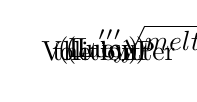
\begin{tikzpicture}[baseline=(root.base)]
        \Tree 	[.\node(root){VolitionP};
                    [.DP \edge[roof]; \node (fin) {(Lucy)}; ]
                    [.Volition$'$
                        Volition
                        [.InitiationP
                            [.DP \edge[roof]; \node (int) {(Lucy)}; ]
                            [.Initiation$'$
                                Initiation
                                [.StateP
                                    State
                                    [.ChangeP
                                        [.DP \edge[roof]; \node (sbj) {the butter}; ]
                                        [.Change$'$
                                            Change
                                            [.OrientedP
                                                Oriented
                                                [.VP \edge[roof]; $\sqrt{melt}$ ]
                                            ]
                                        ]
                                    ]
                                ]
                            ]
                        ]
                    ]
                ]
    \end{tikzpicture}}
\end{figure}

Thus the VISCO approach maintains, in essence, the Burzio-type approach to
understanding split intransitive behaviours, but combines it with a more
fine-grained understanding of syntactic structure. Some reasons for preferring
this more fine-grained syntactic structure are presented in the next two
subsections, which identify two particular kinds of problem with the
traditional \isi{unaccusative hypothesis}, which it is argued the VISCO approach is
able to overcome.

\subsection{The problem of binary classification}\label{sec:baker:3.4}

\subsubsection{Introduction}\label{sec:baker:3.4.1}

As noted, \citet{Perlmutter1978} and much subsequent work divides intransitives
into two main classes, unergatives and unaccusatives. This section will present
various ways in which this binary classification proves to be problematic. It
also discusses some suggested solutions, arguing that these have weaknesses but
that these can be overcome by incorporating their insights into the VISCO
model.

\subsubsection{Ambiguity in classification criteria}\label{sec:baker:3.4.2}

Given Perlmutter’s criteria for distinguishing unergatives and
unaccusatives\linebreak given in (\ref{ex:19.19}--\ref{ex:19.20}) above, one
issue arises with predicates that satisfy criteria from both classes. For
example, volitional acts are supposed to be expressed by unergatives, but verbs
like \emph{fall}, \emph{slide} and \emph{disappear} are meant to be
unaccusative\is{unaccusativity}. What happens, then, when verbs in this latter
set describe volitional events: a deliberate act of falling or sliding, for
example?

Perlmutter discusses this sort of verb (\citeyear[163--164]{Perlmutter1978}),
considering oppositions such as the following:

\ea\label{ex:19.26}
    \ea The wheels slid on the ice.
    \ex Joe slid into third base. \parencite[163--164]{Perlmutter1978}
    \z
\z
(\ref{ex:19.26}a) (non-volitional) is analysed as unambiguously unaccusative;
Perlmutter suggests (\ref{ex:19.26}b) is either unergative\is{unergativity} on
account of its volitionality or a biclausal causative – presumably something
like the following, where the embedded\linebreak clause is
unaccusative\is{unaccusativity} like (\ref{ex:19.26}a) above:

\ea\label{ex:19.27}
    [Joe \textsc{cause} [slid Joe into third base]]
\z
Implicit in the first suggestion is that the volitionality of a predicate might
somehow \enquote{override} its unaccusative\is{unaccusativity} status and lead
to it being classified as unergative\is{unergativity}, but this is not
developed by Perlmutter. (\ref{ex:19.27}) is arguably an over-complex
representation of the sentence and requires an analysis (likewise not provided
by Perlmutter) of why the second \emph{Joe}, or whatever element occupies that
position, is not pronounced.

Unergative/unaccusative ambiguities like these lead Perlmutter to not classify
certain classes of verbs at all: he mentions verbs of motion, presumably verbs
like \emph{go} and \emph{arrive}, as amongst those he chooses not to
categorise.

Ambiguities of classification have proven to be a continuing problem in the
theory of \isi{split intransitivity}. Ongoing research in the years following
\citegen{Perlmutter1978} article identified many so-called \enquote{mismatches},
where the classes of unaccusatives and unergatives appeared to differ between
languages – or where different purported diagnostics of unaccusativity
\emph{within} a language identified different classes. An important early
work in this regard is \citet{Rosen1984}. Rosen shows, for example, that the
verbs meaning `to sweat' show unaccusative\is{unaccusativity} properties in Choctaw
(occurrence with accusative\is{accusative case} pronouns) but unergative\is{unergativity} properties in \ili{Italian}
(occurrence with auxiliary\is{auxiliaries} \HAVE):

\begin{multicols}{2}
\ea Choctaw \parencite[62]{Rosen1984}\\
    \gll Sa-laksha.\\
    \Fsg.\Acc-sweat\\
    \glt \enquote*{I sweated.}\\
\ex  \ili{Italian} \parencite[62]{Rosen1984}\\
    \gll Ho sudato.\\
    have.\Fsg{} sweated\\
    \glt \enquote*{I sweated.}\\
\z\end{multicols}

\noindent I will now discuss some particular sorts of problems in unergative/unaccusative
classification which can be observed to occur: firstly, where the unergative
and unaccusative\is{unaccusativity} classes in a given language appear to overlap on the basis of
standard diagnostics (\sectref{sec:baker:3.4.3}); secondly, where certain verbs cannot be reliably
placed in either class according to the diagnostics (\sectref{sec:baker:3.4.4}); thirdly (and
relatedly), the problem of verbs which do not behave as expected in relation to
the class to which they are supposed to belong (\sectref{sec:baker:3.4.5}); and fourthly, the
matter of cross-linguistic variation (\sectref{sec:baker:3.4.6}). I will discuss some existing
proposed solutions to these issues (where relevant), some problems with these
solutions, and also the solutions which are possible in the VISCO approach.

\subsubsection{Overlaps}\label{sec:baker:3.4.3}

One problem with traditional approaches to unaccusativity occurs with apparent
overlaps between unergative\is{unergativity} and unaccusative\is{unaccusativity} classes. This occurs, for example,
when diagnostics of telicity are considered to diagnose unaccusativity –
various authors have connected telicity to unaccusativity in various languages
(such as \citealt{Zaenen1988}, \citealt{Borer2005}), including
\citet[227]{Schoorlemmer2004} for \ili{English}. Certainly many
\enquote{unaccusative} verbs do not readily allow \enquote{atelic} readings, as
shown by their incompatibility with \emph{for hours} in contexts like the
following:

\ea
    \ea[*]{Lucy arrived for hours.}
    \ex[*]{Chris died for hours.}
    \ex[*]{The window broke for hours.}
    \z
\z
By contrast, all \enquote{unergative} verbs allow \emph{for hours} in
parallel contexts:

\ea
    \ea Lucy coughed for hours.
    \ex Chris swam for hours.
    \ex Harry played for hours.
    \z
\z
However, many \enquote{unaccusative} verbs do allow \emph{for hours} just as
readily:

\ea
    \ea The butter melted for hours.
    \ex The wood burned for hours.
    \z
\z
The class of verbs which allow \emph{for hours} in this sort of sentence,
then, overlaps with the classes identified as \enquote{unergative} and
\enquote{unaccusative} by the other diagnostics. One way around the problem is
simply to deny that telicity relates to unaccusativity at all. This is the
approach taken by \citet{LevinRappaportHovav1995} (henceforth L\&RH), which
remains one of the most important works on \isi{split intransitivity} to date.  They
show that not all \enquote{unaccusative} verbs are telic (pp.\ 172--173), which is
the same position taken here. But it is not therefore possible on their
approach to capture a link between telicity and argument structure, which is
problematic as many authors (for example, \citealt{Tenny1987},
\citealt{Borer2005}) have presented evidence for just such a link, in English
and other languages. For instance, \citet{Kiparsky1998} links telicity to case
in \ili{Finnish}:

\ea \ili{Finnish}
    \ea
        \gll    Ammuin   karhu-\textit{a}.\\
               I.shot   bear-\Part\\
        \glt   \enquote*{I shot at the bear.}\\
    \ex
        \gll    Ammuin   karhu-\textit{n}.\\
                I.shot   bear-\Acc\\
        \glt   \enquote*{I shot the bear.}\\
    \z
\z
Case is of course often related to the relative positions of arguments, which
suggests it is appropriate to link telicity to argument structure. This is lost
on L\&RH’s approach.

A L\&RH-style approach which did make reference to telicity might not fare
much better, however. For them, verbs must classify as either unergative\is{unergativity} or
unaccusative (see \sectref{sec:baker:3.5} for discussion of how this is achieved): they
would not capture how a verb like \emph{melt} patterns with \emph{break}
(unaccusative) in terms of the resultative construction but with \emph{work}
(unergative) in terms of the \emph{for hours} diagnostic. We cannot get
around this problem by positing that \emph{melt} is unergative\is{unergativity} when it is
atelic but unaccusative\is{unaccusativity} when telic. It still shows the properties of an
\enquote{unaccusative} in clearly atelic contexts, for example it allows the
resultative construction (a prototypical diagnostic of unaccusativity;
restricted to [$-$\Initiation{}, $+$\Change{}] verbs):

\ea The butter melted soft for hours.
\z
This sort of pattern is not an issue on the VISCO approach, however. On this
approach \emph{for hours} and the other diagnostics are simply sensitive to
separate features, separately encoded in syntactic structure, and overlaps
between classes are not a problem.

The VISCO approach can be further compared in this regard to another important
strand of work on split intransitive phenomena, labelled the
\enquote{semantic approach} by L\&RH (§1.2.2). Whilst Perlmutter’s original
conception of unaccusativity made reference to both syntax and semantics, the
semantic approach attempts to explain split intransitive patterns in terms of
semantics alone, without reference to syntactic notions such as the structural
positions of arguments.\footnote{L\&RH also identify the \enquote{syntactic
approach} (§1.2.1), exemplified with \citet{Rosen1984}. Contrary to L\&RH’s
implication, however, this is not the direct opposite to the semantic approach
– while Rosen argues that unaccusative\is{unaccusativity} behaviours are not wholly determined by
semantics, she still seems to allow some role for it.}  This approach denies
that the difference between unergative\is{unergativity} and unaccusative\is{unaccusativity} predicates relates to
syntactic structure, and instead claims that the distinction between the two is
entirely due to the sensitivity of the diagnostic constructions to different
semantic values of the predicate. Works which adopt this sort of approach
include \citet{Valin1990} and \citet{Zaenen1993}. Zaenen, for example,
argues that the availability of prenominal past \isi{participles} in
\ili{Dutch} is sensitive to telicity (\ref{ex:19.35}), whereas the availability
of impersonal passives is sensitive to \enquote{protagonist control}
(\ref{ex:19.36}):

\ea\label{ex:19.35} \ili{Dutch} (adapted from \citealt[140]{Zaenen1993})
    \ea[]{%
        \gll de   gevallen   jongen\\
             the   fallen   boy\\\hfill[$+$\textsc{telic}]
         \glt  \enquote*{the boy who has fallen}\\}
    \ex[*]{%
        \gll    de   gewerkt  man\\
             the   worked     man\\\hfill[$-$\textsc{telic}]
         \glt   \enquote*{the man who has worked}}
    \z
\ex \label{ex:19.36} \ili{Dutch} (adapted from \citealt[131]{Zaenen1993})
    \ea[]{%
        \gll Er   werd   hard   gewerkt.\\
        there   became   hard   worked\\\hfill[$+$\textsc{control}]
        \glt \enquote*{There was hard work.}}
    \ex[*]{%
        \gll Er werd   gebloed.\\
            there   became   bled\\\hfill[$-$\textsc{control}]
        \glt \enquote*{There was bleeding.}}
    \z
\z
The semantic approach does not predict that all purported
\enquote{unaccusatives}, or all purported \enquote{unergatives}, need behave in
the same way. Different diagnostics may pick out separate, if overlapping,
groups of verbs. This insight is retained in the VISCO approach. In addition to
the examples discussed above, observe for example that various verbs allow
prenominal past \isi{participles} but disallow resultatives:\largerpage[-1]

\ea Prenominal past \isi{participles}
    \ea the burned bacon
    \ex the recently arrived recruits
    \ex the departed visitor
    \z
\ex Resultatives
    \ea[]{The bacon burned black.}
    \ex[*]{Lucy arrived tired. [intended meaning: \enquote*{Lucy became tired as a result of arriving}]}
    \ex[*]{Chris departed tired. [intended meaning: \enquote*{Chris became tired as a result of departing}]}
    \z
\z
An approach which makes reference to semantics can elegantly account for
mismatches of this sort simply by postulating that the two constructions are
sensitive to different sets of semantic features ([$-$\Initiation{},+\Change{}] for
resultatives; [$+$\Change{}] alone for prenominal past \isi{participles}). This is
exactly what is done in the VISCO approach, somewhat following the semantic
approach. Different diagnostics pick out different classes of verbs, summarised
for \ili{English} in \Cref{tab:key:19.1} (for further discussion see
\citealt{Baker2018,Baker2019}).\footnote{Though the discussion here focuses on
English, similar remarks can be made about other languages.}\largerpage[-2]

\begin{table}
\begin{tabular}{ll}
\lsptoprule
Diagnostics & Principal intransitives identified\\\midrule
V \emph{away}, V \emph{one’s way} into, suffix \emph{{}-er} & [$-$\Change{}, $-$\State{}]\\
Cognate objects, prefix \emph{out}{}- & [$-$\Change{}, $-$\State{}, (+\Volition)]\\
Resultatives, causatives & [$+$\Change{}, $-$\Initiation{}]\\
Prenominal past \isi{participles} & [$+$\Change{}]\\
\emph{for hours} & [$-$\Oriented{}]\\
\lspbottomrule
\end{tabular}
\caption{Summary of classes identified by \ili{English} split intransitivity
diagnostics}\label{tab:key:19.1}
\end{table}

A further advantage of the semantic approach is its ability to capture
straightforwardly the semantic basis of split intransitive behaviours. Many
diagnostics pick out a set of verbs which can be defined in relatively
clear-cut ways. Thus, each class has a well-defined semantic characterisation,
unlike either of the\linebreak \enquote{unergative} or \enquote{unaccusative} classes.
For example, as I have argued in \textcite{Baker2016,Baker2018,Baker2019} and
also discussed above, a number of diagnostic constructions in \ili{English} are
acceptable for the most part only with those intransitives that can be
characterised as [$-$\State{}, $-$\Change{}] (like \emph{talk}, cf. [$+$\State{}]
\emph{remain} and [$+$\Change{}] \emph{arrive}):\footnote{It is true that these
    constructions are sometimes found with unaccusatives: e.g.

\ea The butter melted into the toast.
\ex Lucy was freezing away outside in the snow.
\ex The play died a death.
\ex survivor\z
But such forms are generally sporadic exceptions and mostly do not seem to
reflect any underlying generalisation; speakers’ judgements regarding them are
often weaker.}

\ea
    \ea Lucy talked/*remained/*arrived her way into the room.\\
    \ex Lucy was talking/*remaining/*arriving away.\\
    \ex Lucy talked the talk/*remained the remaining/*arrived the arrival.\\
    \ex talker, *remainer, *arriver\\
    \ex Lucy outtalked/*outremained/*outarrived Chris.
    \z
\z
On the other hand, as again already mentioned, the causative alternation and
the resultative construction seem to be limited to intransitives
characterisable as [$+$\Change{}, $-$\Initiation{}]:

\ea
    \ea[]{Lucy burned the bacon. \hfill[$+$\Change{}, $-$\Initiation{}]}
    \ex[*]{Lucy arrived Chris.   \hfill[$+$\Change{}, $+$\Initiation{}]}
    \ex[*]{Lucy talked Chris.    \hfill[$-$\Change{}, $+$\Initiation{}]}
    \z
\z

\ea
    \ea[]{The bacon burned black.}
    \ex[*]{Lucy arrived tired. [intended meaning: \enquote*{Lucy became tired as a result of arriving}]}
    \ex[*]{Lucy talked tired. [intended meaning: \enquote*{Lucy became tired as a result of talking}]}
    \z
\z
A semantic approach to these phenomena, making no reference to syntactic
grammatical relations or argument positions, would be able to capture the
behaviour of these constructions by reference to the semantic features alone.
This has the apparent advantage of not having to make additional reference to
an additional concept of \enquote{unaccusativity}, thus allowing for an
apparently simpler grammar. The VISCO approach shares this advantage, defining
classes in terms of semantic features with no separate concept of
unaccusativity.

\hspace*{-0.55959pt}However, the semantic approach misses some important generalisations which
appear to connect \isi{split intransitivity} to argument structure.
\textcite[11--12]{LevinRappaportHovav1995} discuss the example of prenominal
past \isi{participles}, which may only modify what would be \enquote{internal
arguments} in the equivalent clausal constructions, under a standard
Burzio-type approach to syntactic structure:

\ea
    \ea Internal argument of transitive: \emph{a badly written letter}
    \ex Internal argument of intransitive (unaccusative): \emph{a recently appeared book}
    \ex External argument of transitive: *\emph{a much-painted artist}
    \ex External argument of intransitive (unergative): *\emph{a hard-worked lawyer} (L\&RH: 11)
    \z
\z
As was exemplified in \sectref{sec:baker:3.3}, the ability to capture this sort of parallel
between intransitives and transitives is an important strength of the
traditional \isi{unaccusative hypothesis}, and indeed of any implementations of it
which make reference to grammatical relations or argument positions. L\&RH
argue, however, that the semantic approach fails to account for such parallels
satisfactorily, as there is no single semantic notion that all
\enquote{internal arguments} have in common -- \citegen{Valin1990} appeal to an
\enquote{undergoer} macrorole, they claim convincingly, cannot be considered
truly semantic but rather a generalisation over a number of specific semantic
roles.  This, then, is a major weakness of the semantic approach.

The VISCO approach, however, overcomes this weakness. As discussed in \sectref{sec:baker:3.2}, it
is able to account for parallels between transitives and intransitives in
structural terms. However, because it adopts a more fine-grained approach to
the structure of the thematic domain of the clause, and because this structure
is explicitly connected to semantic features ([$\pm$\Volition{}],
[$\pm$\Initiation{}] etc., valued on the functional heads\is{functional items}), it is also able to
take into account the semantic basis of split intransitive patterns as
effectively as the traditional semantic approaches.

Another partial solution to the issue of overlaps between classes may be found
in the work of \citet{Ramchand2008}, who proposes the following structure for
the thematic domain – a fairly significant departure from traditional
assumptions:

\ea
    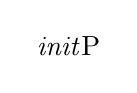
\begin{tikzpicture}[baseline=(root.base)]

        \Tree 	[.\node(root){\emph{init}P};
                    \emph{init}
                    [.\emph{proc}P
                        \emph{proc}
                        [.\emph{res}P
                            \emph{res}
                            {}
                        ]
                    ]
                ]

    \end{tikzpicture}
\z
Arguments can be merged in the specifier positions of any of these three heads
(the complement positions of \emph{proc} and \emph{res} are also available for
arguments, but these do not seem to be filled in one-argument verbs). An
argument merged in Spec,\emph{init}P is termed an \enquote{\textsc{initiator}},
that in Spec,\emph{proc}P an \enquote{\textsc{undergoer}} and that in
Spec,\emph{res}P a \enquote{\textsc{resultee}}. The same argument can be merged
in more than one of these positions: thus for example \emph{run} is an
[\emph{init}, \emph{proc}] verb and its argument is both \textsc{initiator} and
\textsc{undergoer}, and \emph{arrive} is [\emph{init}, \emph{proc}, \emph{res}]
so its argument is simultaneously \textsc{initiator},
\textsc{undergoer} and \textsc{resultee}, whereas
\emph{roll} has only a \emph{proc} projection and thus its argument is only
an \textsc{undergoer.} Thus, there are not just two possible configurations for
intransitive predicates (as suggested under the traditional unaccusative
hypothesis), but multiple possibilities.

As a result of this, Ramchand’s approach can account for certain of the
discrepancies between \isi{split intransitivity} diagnostics. Not only may the
arguments of different predicates appear in more than two different positions –
which itself allows for split intransitive diagnostics sensitive to argument
structure to pick out more than two classes – the argument of a single given
predicate may appear in multiple different positions at once, allowing it to be
picked out by multiple argument-structure-sensitive diagnostics even if they
are sensitive to different factors.

For example, the causative alternation is on Ramchand’s analysis restricted to
those intransitive verbs which lack an \emph{init} component. This is
independent of telicity, which is connected (in part) to the presence or
absence of \emph{res}. Ramchand thus accounts for both diagnostics in
structural terms, without making the false prediction that (for example) all
intransitives with causative alternants are telic. This prediction is shown to
be false by examples such as the following:

\ea
    \ea The lollipops melted.
    \ex Lucy melted the lollipops.
    \z
\ex
    The lollipops melted for hours.
\z
However, there are some patterns Ramchand’s approach does not so obviously
account for. For example, it does not identify the [$+$\Change{}] class, which I
have argued in favour of in \sectref{sec:visco}.\footnote{A reviewer suggests that the
    [$+$\Change{}] property as identified by the prenominal past participle
    diagnostic might be related to the non-finite participle morphology, rather
    than as part of the extended structure of finite verbs. It seems to me most
    economical to assume that the structure of finite and non-finite forms does
    not differ in this way; in any case, this does not account for the apparent
operation of the [$\pm$\Change{}] feature in other ways.}  In \citet{Baker2018}, I
identify this and other problems, arguing at length the patterns are more
readily accounted for in terms of a more elaborated sequence of heads. The
parallels between Ramchand’s and my approach are, however, very strong, even if
the particular heads identified are different.

The VISCO hierarchy approach, then, allows diagnostics to pick out overlapping
classes without encountering these issues. Recall that verbs like \emph{melt}
pattern both with verbs like \emph{work} (in terms of diagnostics of telicity
like \emph{for hours}) and with verbs like \emph{break} (in terms of other
diagnostics: resultatives, causatives, prenominal past \isi{participles}). If we
assume all of these diagnostics are connected to argument structure, this is
difficult – if not impossible – to account for on the assumption that there are
only two available argument positions in intransitives. Either telicity or the
other diagnostics must be sensitive to argument structure on this more
traditional approach; it does not seem that they can both be. However, if we
allow for the possibility of multiple argument positions – and specifically
multiple \enquote{internal} argument positions – we are able to account for
both sets of phenomena in argument structure terms.

\subsubsection{Non-classified verbs}\label{sec:baker:3.4.4}

This section considers the problem, for the traditional unaccusative
hypothesis, of predicates which apparently cannot be classified as unergative
or unaccusative\is{unaccusativity}. For the \isi{unaccusative hypothesis} to be tenable, there should be
some way of identifying any given intransitive predicate one way or the other.
This is desirable not only from a theoretical perspective (we do not wish to be
making claims about the status of predicates on an ad hoc basis) but also from
an acquisitional one:\is{language acquisition} the language learner needs some method by which verbs can
be identified as belonging to one class or the other.

The obvious method to determine the status of predicates as unergative\is{unergativity} or
unaccusative is via the various \enquote{unaccusativity diagnostics}, a number
of which have already been discussed. These are morphological or syntactic
constructions which permit some intransitives to participate but disallow
others. But matters are not as straightforward as might be hoped. Consider, in
English, verbs denoting states. As discussed above, and illustrated in more
detail immediately below, these are rather consistently disallowed with both
constructions purportedly diagnostic of unergatives (\ref{ex:19.46}) and those
diagnostic of unaccusatives (\ref{ex:19.47}):\footnote{\emph{Remain} and many other
    statives are permitted with locative inversion and
    \emph{there}{}-insertion:

\ea In the room remained a man.
\ex There remained a man.\z
However, I do not consider these true diagnostics of argument structure: see
\textcites[Ch.\ 6]{LevinRappaportHovav1995,Baker2018,Baker2019}.}

\ea\label{ex:19.46}
    \ea[*]{Lucy remained her way into the room.}
    \ex[*]{Lucy was remaining away.}
    \ex[*]{Lucy remained a remaining.}
    \ex[*]{remainer}
    \ex[*]{Lucy outremained Chris.}
    \z
\z

\ea\label{ex:19.47}
    \ea[*]{Lucy remained happy. [intended meaning: \enquote*{Lucy became happy as a result of remaining}]}
    \ex[*]{Lucy remained Chris. [intended meaning: \enquote*{Lucy made Chris remain}]}

    \ex[*]{the remained man}
    \z
\z
Similar observations can be made of many other verbs denoting states:
\emph{stay}, \emph{last}, \emph{survive}, \emph{persist}; \emph{sit},
\emph{stand} (in their stative senses), etc. It is true that these do
sporadically allow certain of the diagnostic constructions (e.g.
\emph{survivor}, \emph{outstay}; \emph{Lucy stood the statue in the corner}),
but such behaviours do not seem to form part of any general pattern and it is
not clear that they do much to resolve the issue.

There is one diagnostic that does group statives with other verbs: that of
telicity. Statives can freely occur with phrases like \emph{for hours}:

\ea
    Lucy remained for hours.
\z
But as discussed in \sectref{sec:baker:3.4.3}, the classes identified by this diagnostic do not
line up neatly with those picked out by the other diagnostics: both
\enquote{unergative} and \enquote{unaccusative} verbs can occur with \emph{for
hours}, so the telicity diagnostic does not solve the problem.

Of course, it is notionally plausible that the division of predicates into one
or the other class derives from some sort of innate knowledge. Such knowledge
would most probably be specific to the language faculty – it is hard to see how
the mechanisms which allow the linking of semantics to grammatical relations or
syntactic argument structure could have any non-linguistic applications.
However, appeals of this sort to \enquote{Universal Grammar} (\glsunset{UG}\gls{UG}) are not very
compatible with a minimalist approach, which favours an \enquote{impoverished}
view of UG\@. This thus avoids the methodological error of appealing to
innateness too readily, and failing to seek out deeper explanations.  \gls{UG}\is{Universal Grammar} is
predicted to contain as little as possible, and we ought not to be placing the
mechanisms for distinguishing unergatives from unaccusatives within it if
better options are available. That is, we ideally do not want a \gls{UG}\is{Universal Grammar} principle
which states \enquote{Intransitive predicates denoting changes and states are
unaccusative; others are unergative} or the like.

This sort of \gls{UG}\is{Universal Grammar} approach would also run into problems with cross-linguistic
variation. If, as seems to be the case, languages vary to some extent as to how
they classify intransitives, then it would seem \gls{UG}\is{Universal Grammar} would only provide partial
information as to how this classification is to proceed. This would leave us
with the problem of determining what information is, and is not, in \gls{UG}\is{Universal Grammar} – a
problem which is by no means easy to solve. This problem is perhaps
particularly apparent with intransitives denoting states. State verbs often
show a great deal of language-internal variation and apparent lexical
idiosyncrasy with regard to \isi{split intransitivity} diagnostics. In \ili{Dutch}, for
example, some state verbs occur with \HAVE{} and others with \BE:

\ea \ili{Dutch} \parencite[870]{Sorace2000}
    \ea
        \gll    Het   beeldje \textit{heeft} op   de   tafel   gestaan.\\
                the   picture   has   on   the   table   stood\\
        \glt    \enquote*{The picture stood on the table.}
    \ex
        \gll   Sofie \textit{is} een   geode   docente   gebleken.\\
               Sofie is a   good   teacher   seemed\\
        \glt   \enquote*{Sofie seemed a good teacher.}
    \z
\z
Similar observations can be made with regard to case marking of statives in
\ili{Basque} and \ili{Georgian} \parencite{Baker2018}. This suggests
\gls{UG}\is{Universal Grammar} does not provide much if any help in the
classification of these verbs into one of the two purported groups.

Given all this, how can the language learner (or the linguist) determine
wheth\-er \ili{English} stative verbs are unergative\is{unergativity} or unaccusative? They have
generally been assumed to belong to the latter class (see
\citealt{Perlmutter1978}: 162–163), but as we have seen there is little
positive evidence in support of this, only the negative evidence that they do
not generally pattern with the \enquote{unergatives}.

Another possibility is that \gls{UG}, or general cognitive procedures, allow for some
sort of \enquote{default rule}, whereby verbs for which there is no positive
evidence as to their status are classified into one particular group. However,
it is not clear (at least at present) how we might determine which of the two
groups is the default, suggesting we ought not to pursue this path if an
alternative can be found.

The VISCO approach may be just such an alternative. It does not run into
problems with [$+$\State{}] intransitives. As there is no requirement on this
approach for these verbs to be classified into one of just two groups, the fact
that the diagnostics do not allow us to do so is not problematic. Rather,
stative verbs can simply be grouped into a class of their own.

\subsubsection{Exceptional verbs}\label{sec:baker:3.4.5}

Another problem for the \isi{unaccusative hypothesis} concerns verbs which, having
been classified as either unergative\is{unergativity} or unaccusative\is{unaccusativity}, fail to show particular
behaviours expected of the group in question. In \ili{English}, this is particularly
problematic for the unaccusative\is{unaccusativity} class. Because not all purported
\enquote{unaccusatives} behave in the same way in relation to the diagnostics,
authors working within the \isi{unaccusative hypothesis} framework must posit reasons
for the \enquote{exceptional} behaviour of certain sorts of predicate. Thus,
for example, \citet{LevinRappaportHovav1995} provide arguments for the
incompatibility of resultatives with directed motion (§2.3.2) and stative
(§2.3.3) intransitives, and for the incompatibility of the causative
alternation with verbs of existence and appearance (§3.3, see especially p.
126). This sort of approach – whereby some members of a class whose members are
able to enter into a given construction for one reason (such as the presence of
an internal argument\slash absence of an external argument) are ruled out in that
construction for some other reason – is not inherently problematic. L\&RH’s
use of it in this instance, however, runs into various problems.

Firstly, note again that the resultative construction and the causative
alternation are available in \ili{English} with very almost the same class of verbs
(see also \citealt{Baker2018,Baker2019}):\footnote{The major exception is the
    class of verbs comprising \emph{redden}, \emph{blacken}, \emph{ripen} etc.\
    which allow causatives but not resultatives:

\ea[]{The wood blackened.}
\ex[]{The fire blackened the wood.}
\ex[*]{The wood blackened black.}
\z

One explanation for this property is that the result state (\emph{red},
\emph{black}, \emph{ripe} etc.) incorporates directly into the verbal element
\emph{-en}.}

\ea
    \ea[]{The butter melted soft.}
    \ex[]{The wood burned black.}
    \ex[]{The window broke into pieces.}
    \ex[*]{Lucy arrived tired. [intended meaning: \enquote*{Lucy became tired as a result of arriving}]}
    \ex[*]{Lucy persisted happy. [intended meaning: \enquote*{Lucy became happy as a result of persisting}]}
    \z
\ex
    \ea[]{Chris melted the butter.}
    \ex[]{Chris burned the wood.}
    \ex[]{Chris broke the window.}
    \ex[*]{Chris arrived Lucy.}
    \ex[*]{Chris persisted Lucy.}
    \z
\z
This correspondence occurs even with verbs which otherwise appear to be
idiosyncratic exceptions to the non-availability of these
constructions:

\ea
    \ea[*]{Lucy died dead. [intended meaning: \enquote*{Lucy became dead as a result of dying}]}
    \ex[*]{Chris died Lucy.}
    \z
\z
L\&RH’s approach, however, does not account for this generalisation of close
correspondence between the classes picked out by the two diagnostics. This
correspondence cannot be explained simply by claiming that the constructions
are only available with \enquote{unaccusatives}, because the pattern is subtler
than that: not all intransitives claimed to have internal arguments allow the
two constructions. Further, L\&RH’s arguments for the incompatibility of
resultatives with certain \enquote{unaccusatives} do not generalise to the
incompatibility of these same verbs with the causative alternation (and vice
versa). The inherent delimitation of directed motion verbs may be a
satisfactory account of their non-occurrence with resultatives (L\&RH: §2.3.2),
but it does not seem relevant to the causative alternation; similarly, while it
may be reasonable that there are no such things as delimited states and hence
no resultatives of statives, as resultatives (§2.3.3), this line of argument
does not obviously extend to the lack of causative alternants of stative forms.

Likewise, L\&RH’s argument for the non-occurrence of causative alternants of
verbs of existence and appearance does not account for the non-occurrence of
these verbs with resultatives:

\ea
    \ea[*]{The ghost appeared white. [intended meaning: \enquote*{The ghost became white as a result of appearing}]}
    \ex[*]{Lucy vanished invisible.}
    \z
\z
L\&RH argue (p. 126) that these verbs lack causative alternants because they have
neither external nor internal causes, but this is irrelevant to whether they
allow resultatives on their analysis (though cf.\ \citealt{Ramchand2008};
\citealt{Baker2018,Baker2019}). They do not provide any argument for the
non-occurrence of causatives with other \enquote{unaccusatives}.

To reiterate, then, L\&RH fail to capture significant similarities between the
behaviour of these two diagnostics. In this respect, then, they can be argued
to do less well than the \enquote{semantic}-type approaches, which are able to
identify features the verbs allowing resultatives and causatives have in common
([$+$\Change{}, $-$\Initiation{}], as I suggested above). The fact that this class
can be identified positively in terms of these features alone, rather than
positing an unaccusative\is{unaccusativity} class and various exceptions, might also seem to
favour something more like a semantic approach – or the VISCO approach. We can
make a similar argument regarding prenominal past \isi{participles}, some examples of
which are as follows:

\ea
    \ea[]{the fallen tree}
    \ex[]{the broken window}
    \ex[*]{the survived man}
    \ex[*]{the been man}
    \ex[*]{the swam athlete}
    \z
\z
L\&RH would have to provide some reason to rule these out with statives,
whereas the VISCO approach need only state that they are restricted to verbs of
change. On this approach, as discussed above, there is no expectation that
different \isi{split intransitivity} diagnostics should all identify more-or-less the
same two classes, and indeed this is not what we observe. Accordingly, there is
a reduced need to explain away the apparent exceptions: the cases where certain
verbs do not behave as their class membership predicts.\footnote{It is true
that there are some [$+$\Change{}, $-$\Initiation{}] verbs that do not allow
resultatives and/or causatives: among them, \emph{die}, verbs of
(dis)appearance and verbs like \emph{redden}, \emph{blacken} etc. There are
also exceptions to the rule that [$+$\Change{}] verbs allow prenominal past
participles (\emph{*the gone man}, etc.). The number of exceptions to be
accounted for is still less than on an approach that treats these constructions
as in principle available with all \enquote{unaccusatives}. See discussion in
\textcite{Baker2018,Baker2019}.}  However, as already noted, the VISCO approach also
has the advantage over traditional semantic approaches in that it nevertheless
connects class membership to syntactic structure and accordingly is able to
account for particular patterns which those other approaches do not.

\subsubsection{Variation between languages}\label{sec:baker:3.4.6}

Variation in split intransitive phenomena has been highlighted by various
authors, for example \citet{Rosen1984} cited above, and more recently in the
work of Sorace (see particularly \citealt{Sorace2000}, forthcoming).
\citet{Sorace2000} describes variation in auxiliary\is{auxiliaries} selection in \ili{German}, \ili{Dutch},
Italian and French: these languages all allow either \BE{} or \HAVE{} as the
auxiliary in the periphrastic perfect, with \BE{} traditionally held to occur with
unaccusatives and \HAVE{} with unergatives. However, the distribution of \BE{} and
\HAVE{} is different in each language. The following examples illustrate:

\ea \ili{French}\\
    \gll Il \textit{a} courru.\\
        he has run\\
    \glt \enquote*{He ran.}
\ex  \ili{German}\\
    \gll Er \textit{ist} gelaufen.\\
    he is run\\
    \glt \enquote*{He ran.}
\z
Sorace shows, however, that this cross-linguistic variation in amenable to
analysis in terms of a hierarchy of semantic categories of intransitive verbs:
the \gls{ASH} or \gls{SIH} \citep{SoraceShomura2001}.  This is given in
\Cref{tab:key:19.2}. Whilst the \enquote{cut-off point} between \HAVE{} verbs and
\BE{} verbs varies between languages, in general categories toward the top of the
hierarchy are associated with \HAVE{} and those toward the bottom with \BE.

\begin{table}
\begin{tabularx}{\textwidth}{QQ}
\lsptoprule
Controlled process (non-motional) & \emph{work}, \emph{play}, \emph{talk \dots{}}\\
Controlled process (motional) & \emph{swim}, \emph{run}, \emph{walk} \dots{}\\
Uncontrolled process & \emph{tremble}, \emph{skid}, \emph{cough}, \emph{rumble} \dots{}\\
Existence of state & \emph{be}, \emph{belong}, \emph{sit} \emph{\dots{}}\\
Continuation of a pre-existing state & \emph{stay}, \emph{remain}, \emph{last}, \emph{survive}, \emph{persist} \dots{}\\
Change of state & \emph{rise}, \emph{decay}, \emph{die}, \emph{grow} \dots{}\\
Change of location & \emph{come}, \emph{arrive}, \emph{leave}, \emph{fall} \dots{}\\
\lspbottomrule
\end{tabularx}
\caption{The \glsdesc{SIH} \parencite{Sorace2000}}\label{tab:key:19.2}
\end{table}
Further research has shown that the \gls{SIH} can be applied to split intransitive
phenomena other than auxiliary\is{auxiliaries} selection (\citealt{Sorace2004}: 263--264,
\citealt{Montrul2005}), although it may not apply in all cases
(\citealt{Baker2013,Baker2018}).

Most theoretical accounts of \isi{split intransitivity} have little to say about
what, if any, cross-linguistic variation should be possible. However, as
Sorace’s work shows, languages not only seem to vary in which predicates show
\enquote{unergative} and \enquote{unaccusative} behaviours, but this variation
appears not to be purely random.

The VISCO hierarchy, however, can be seen as an implementation of the SIH\@.
Categories closer to the top of the \gls{SIH} correspond to positively valued
features of heads towards the top of the VISCO hierarchy, as summarised in
\Cref{tab:key:19.3} (for further discussion see \citealt{Baker2019}).

\begin{table}
\begin{tabularx}{\textwidth}{Qccccc}
\lsptoprule
& \rotatebox{90}{[\Volition{}]} & \rotatebox{90}{[\Initiation{}]} & \rotatebox{90}{[\State{}]} & \rotatebox{90}{[\Change{}]} & \rotatebox{90}{[\Oriented{}]}\\\midrule
Controlled process (non-motional) & + & + & – & – & –\\
Controlled process (motional) & + & + & – & – & –\\
Uncontrolled process & – & + & – & – & –\\
Existence of state & +/– & +/– & + & – & –\\
Continuation of a pre-existing state & +/– & +/– & + & – & –\\
Change of state & +/– & +/– & – & + & +/–\\
Change of location & +/– & +/– & – & + & +\\
\lspbottomrule
\end{tabularx}
\caption{Correspondences between the \gls{SIH} and the features encoded on the heads
    of the VISCO hierarchy}\label{tab:key:19.3}
\end{table}

This enables explanation of why split intransitive patterns show the patterns
of variation they do, something which is not furnished by other theories. This
is most easily illustrated with auxiliary\is{auxiliaries} selection, which is
also the phenomenon best studied with relation to the SIH\@. The generalisation
which can be made is that in languages with a \HAVE\slash\BE{} split amongst auxiliaries
in the periphrastic perfect with intransitives, \BE{} is associated with heads
below a certain point when they bear a positively valued feature (e.g.\ with
\Oriented{} when it bears [$+$\Oriented{}], but not where it bears [$-$\Oriented{}]);
\HAVE{} is then associated with heads bearing a positively valued feature above
that point. The cut-off point in question, however, varies between
languages.\footnote{This does not by itself account for all the patterns
captured by the \gls{SIH}; for further discussion of how this may be done on a
TFH approach see \citet{Baker2018}.}

To briefly summarise this discussion, it has considered the problem of
attempting to divide intransitives into just two groups, which is manifest in
various ways. It has argued that the VISCO approach, which identifies multiple
classes of intransitives in a way which is connected directly to syntactic
structure, is able to overcome this problem where other approaches run into
difficulties.

\subsection{The problem of semantics--syntax linking}\label{sec:baker:3.5}

A further issue with the \isi{unaccusative hypothesis} as originally proposed
concerns the proposed relation between semantics and syntax. The link between
the meaning of an intransitive predicate and that predicate’s status as
unergative or unaccusative\is{unaccusativity} is not nearly as straightforward as might be thought
ideal. The proposed unergative\is{unergativity} and unaccusative\is{unaccusativity} classes each divide into a
number of subgroups, and the semantic characterisations of each are somewhat
heterogeneous: there is no immediately apparent semantic feature that all the
predicates in one of the classes possess and all the others lack. Thus, the
semantic criteria that \citet{Perlmutter1978} provides
(\ref{ex:19.19}--\ref{ex:19.20}) are not necessarily very informative
– in particular, the notion of \enquote{semantic patient} (\ref{ex:19.20}b) is
unhelpfully vague. And some of the classifications seem rather arbitrary – why,
for example, should \enquote{involuntary bodily processes} be
unergative\is{unergativity} rather than unaccusative?

This problem is overcome somewhat by \citet{LevinRappaportHovav1995}.
Considering a number of diagnostics in a high level of detail, primarily
although not exclusively in regard to \ili{English}, L\&RH argue in favour of a
traditional interpretation of unaccusativity, where the two classes of
intransitive predicates (unergative and unaccusative) are both semantically
determined and syntactically represented.

The mapping of semantics to syntax on L\&RH’s approach is achieved via
\enquote{linking rules} (Ch.\ 4). The rules that L\&RH identify are as follows:

\ea\label{ex:19:54}
    \ea\label{ex:19:54a} Directed change linking rule\\ \enquote{The argument of a verb that corresponds to the entity undergoing the directed change described by that verb is its direct internal argument.} (p. 146)
    \ex\label{ex:19:54b} Existence linking rule\\ \enquote{The argument of a verb whose existence is asserted or denied is its direct internal argument.} (p. 153)
    \ex\label{ex:19:54c} Immediate cause linking rule\\ \enquote{The argument of a verb that denotes the immediate cause of the eventuality described by the verb is its external argument.} (p. 135)
    \ex\label{ex:19:54d} Default linking rule\\ \enquote{The argument of a verb that does not fall under the scope of any of the other linking rules is its direct internal argument.} (p. 154)
    \z
\z
To summarise, with examples of verbs whose arguments are typically subject to
each rule:

\ea\label{ex:19:55}
    \ea\label{ex:19:55a} argument undergoing directed change → direct internal argument\\\hfill e.g.\ \emph{break}
    \ex\label{ex:19:55b} argument whose existence asserted/denied → direct internal argument\hfill e.g.\ \emph{appear}
    \ex\label{ex:19:55c} immediate cause → external argument\hfill e.g.\ \emph{play}
    \ex\label{ex:19:55d} other argument → direct internal argument\hfill e.g.\ \emph{bounce}
    \z
\z
These rules are ordered (L\&RH: §4.2). Thus, for example, the directed change
linking rule (\ref{ex:19:54a}, \ref{ex:19:55a}) takes precedence over the immediate cause linking rule
(\ref{ex:19:54b}, \ref{ex:19:55b}) in at least some languages (L\&RH: 159–164, 166). Thus an entity
which both undergoes a direct change and is an immediate cause of the
eventuality is represented by an internal argument, not an external one. This
is apparent, for example, in the case of \ili{Italian} \emph{cadere} \enquote*{to
fall} which takes auxiliary\is{auxiliaries} \emph{essere} \enquote*{to be} (associated with
unaccusatives) even when agentive (L\&RH: 163):

\ea \ili{Italian}\\
    \gll Luigi   è   caduto   apposta.\\
        Luigi   is   fallen   on.purpose\\
    \glt \enquote*{Luigi fell on purpose.}
\z
In summary, on L\&RH’s approach intransitive predicates with an immediate cause
argument are unergative\is{unergativity} \emph{unless} that argument also undergoes a directed
change or has its existence asserted or denied. All other intransitives are
unaccusative.

The principal advantage, then, of L\&RH’s approach – as opposed to previous
attempts to characterise unaccusativity – is an explicit characterisation of
the different behaviour of different intransitive predicates in semantic terms,
whilst however directly relating these behaviours to the syntactic property of
the position of arguments. L\&RH are thus able to maintain certain advantages
of the \enquote{semantic} approach, whilst overcoming some of its weaknesses by
building on existing insights into syntactic determinants of split intransitive
phenomena. Furthermore, the semantic characterisation it presents is relatively
straightforward~– relying only on the concepts of \enquote{direct change},
\enquote{immediate causation} and \enquote{assertion\slash denial of existence}. This
compares favourably to the numerous semantic categories identified by
\citet{Perlmutter1978}, allowing significant generalisations to be made as to
which predicates fall in which class.

The linking rules approach is not without weaknesses of its own, however. Some
of these concern the rules themselves (I will discuss other weaknesses
subsequently). Now, it seems undeniable that we need some way of linking
semantics to syntax if \isi{split intransitivity} is indeed sensitive to both. The
idea of linking rules is not problematic per se. But the specific forms of the
rules L\&RH suggest are.  They seem largely accurate in describing the classes
of verbs which show \enquote{unergative} and \enquote{unaccusative} behaviours:
though they have some weaknesses even in this regard, which I shall discuss
below. But despite this strength in terms of purely descriptive classification,
it is difficult to come up with independent, explanatory reasons for why they
should have the forms they do. Why are they sensitive to these semantic
factors, and not others? One can think of plenty of other factors which might
just as well be candidates (e.g. volition, sentience, eventivity/stativity,
telicity, affectedness; \enquote{change} as a general concept rather than
directed change specifically).\footnote{L\&RH do discuss (§4.3.1) their
reasoning for rejecting some of these, but this does not explain why language
learners do not posit them.}  The basis for the connections between these
semantic factors and the external/internal argument distinctions are in some
cases similarly unclear. Why, for example, should assertion of existence be a
criterion that yields unaccusatives, and not unergatives? Neither is it easy to
justify the order of the rules. Why should the directed change linking rule
take precedence over the immediate cause linking rule, and not vice versa?

These are problematic issues from an acquisitional perspective.\is{language
acquisition} The forms of
the rules – the semantic features they make reference to, the mapping to
external or internal arguments, their ordering – seem rather arbitrary. This
arbitrariness can only make the acquisition\is{language acquisition} process more difficult,
particularly when the data that are available to help language learners
classify predicates one way or the other are often limited at best.{}

A potential source of evidence for the mapping one way or the other is the
behaviour of arguments of transitive verbs: most clearly for the directed
change linking rule, as transitive arguments which undergo directed changes are
internal arguments, for example \emph{the city} in the following case:

\ea Hannibal destroyed the city.\z
But this reasoning may not generalise to all the rules. True, causes and
\enquote{other} arguments are generally external and internal arguments of
transitives respectively, as in the following example:

\ea Lucy touched the wall.\z
Here, \emph{Lucy} (the external argument) is the immediate cause of the event
and \emph{the wall} (the internal argument) does not come under the scope of
any of the rules. Instances like this could allow the derivation of the
immediate cause and default linking rules. But psych predicates pose a problem,
for example:

\ea Sarah loves Chris.\z
Here, \emph{Sarah} (the external argument) is not necessarily best analysed as
a cause, and \emph{Chris} (the internal argument) may well be. Thus the mapping
to syntactic positions exhibits the opposite pattern from that the linking
rules would generate. It is also not clear if transitives provide any evidence
as to the status of an argument of which existence is asserted or denied.

One solution would be to posit that the linking rules, and maybe their order as
well, are encoded in Universal Grammar. But this does not seem very attractive,
particularly if a better proposal can be made. Most linguists today would
probably reject such a \enquote{rich \gls{UG}} approach.

Ideally, perhaps, learners would have access to some sort of generalised
linking rule format on which all the rules might be based (this might be either
innate or emergent). It is not clear that L\&RH’s linking rules can be reduced
to a satisfactory general format: certainly there does not seem to be one which
overcomes the problems of the arbitrariness of the semantic factors and of
whether each factor maps to external or internal arguments. The issue of the
ordering of the rules would remain problematic in any case.

In \textcite{Baker2018,Baker2019}, however, I propose exactly this sort of
\enquote{generalised linking rule} which, utilising a VISCO-type hierarchy,
overcomes these problems with L\&RH’s rules:

\ea Generalised linking rule\\An argument of which the property [$+$a]
    is predicated is merged in the corresponding Spec,AP.
\z
The properties [$+$a] in question are the features [$+$\Volition{}],
[$+$\Initiation{}] etc.; the corresponding APs are VolitionP, InitiationP, etc.
The general format of the rule allows for much easier acquisition\is{language acquisition}, and there is
no need to order the rules so that certain semantic features take precedence
over others, which obviates the need to justify such a rule ordering, or for
learners to acquire it. (Where two properties are predicated of an argument –
say, [$+$\Initiation{}] and [$+$\Change{}] – that argument is simply merged in both
corresponding positions, as discussed above.)

The VISCO approach does not require us to posit seemingly arbitrary
associations of semantic properties to external or internal argument positions:
on this approach, the two-way division between \enquote{external} and
\enquote{internal} arguments is too simplistic. A related issue does still
present itself, however: why are the heads ordered in the way they are? (Note
that this is a problem here only with the syntactic structure itself – it is
external to the linking rules.) From an acquisitional perspective,\is{language
acquisition} however, it
is not such an issue as it might first appear: there is ample evidence from
transitive and ditransitive clauses\is{ditransitive constructions} for the order of at least some of the heads
in the hierarchy.\footnote{I admit I am not aware of much good
language-internal evidence for the relative order of, firstly, \Volition{} and
\Initiation{} and, secondly, \Change{} and \Oriented{} – though see \sectref{sec:baker:3.4.4} for some
cross-linguistic evidence for the orders posited. It is not clear that much
hinges on which orders the learner adopts in these cases, however.} For
example, \textsc{θ-initiation} arguments always seem to be merged
higher than \textsc{θ-change} ones:

\ea
    \gll    {Hannibal destroyed} {the city}.\\
            \textsc{θ-initiation} \textsc{θ-change}\\
\z
This allows the learner to posit InitiationP as being higher in the structure
than ChangeP. See \citet{Baker2018} for in-depth discussion.

As to why the particular order of heads should have come about in the first
place, I admit I do not have a full explanation. Such deep explanations for the
ordering of heads in syntactic structures are of course a more general issue
not restricted to the particular subpart of sentence structure posited here.
One partial explanation may be that the heads higher in the structure (e.g.
\Volition{}, \Initiation{}) relate more to the properties of the arguments
themselves, whereas the lower heads (e.g. \Change{}, \Oriented{}) say more about the
properties of the event. But this is incomplete and subject to criticism.
Overall, however, the VISCO approach, with the generalised linking rule, allows
a neat way of capturing the linking between semantics and syntax which does not
run into some of the problems encountered by previous accounts.

\section{Conclusion}\label{sec:baker:conclusion}

\citegen{Perlmutter1978} \isi{unaccusative hypothesis} has remained a powerful
idea since its inception. Numerous linguistic phenomena have shown themselves
to be amenable to analysis in terms of unaccusativity. But the hypothesis, and
subsequent implementations and adaptations of it, have also proved problematic
in various ways. My approach to \isi{split intransitivity}, captured in terms
of the VISCO hierarchy, overcomes many of these difficulties by positing more
fine-grained distinctions in syntactic structure. However, it retains key
elements of the original \isi{unaccusative hypothesis}: the idea that split
intransitive behaviours are semantically determined but syntactically encoded,
specifically in terms of \enquote{grammatical relations} here formalised (after
\citealt{Burzio1986} and many others) in terms of argument positions. The VISCO
approach to \isi{split intransitivity} should be seen, therefore, not as a
radical alternative to the \isi{unaccusative hypothesis} but as a development
of it.

\printchapterglossary{}

{\sloppy
\printbibliography[heading=subbibliography,notkeyword=this]
}
%\end{refcontext}
\end{document}
